\section{Force estimation}
%%%%%%%%%%%% MID WAY AGENDA %%%%%%%%%%%%%%
\begin{frame}{Forces}
\begin{itemize}
  	\item Roll, pitch and yaw forces
\end{itemize}
 \begin{figure}[h]
 \centering
 \includegraphics[scale = 0.5]{Endowrist31}
 \label{fig:ewr}
 \end{figure}
\end{frame}


% the license
\begin{frame}{Force estimation}{Model structure}

%\begin{columns}[T]
%\begin{column}{\textwidth}

  \begin{itemize}
    \item Nonlinearities in the EndoWrists dynamics (yaw, pitch)   
    \item Roll force linear
    \item Black-box identification
    \begin{itemize}
      \item Hammerstein-Wiener Model
    \end{itemize}
  \end{itemize}
%\end{column}%
%\hfill%
%\begin{column}{.65\textwidth}

\vspace{3em}
\begin{figure}[H]
\resizebox{0.9\textwidth}{!}{
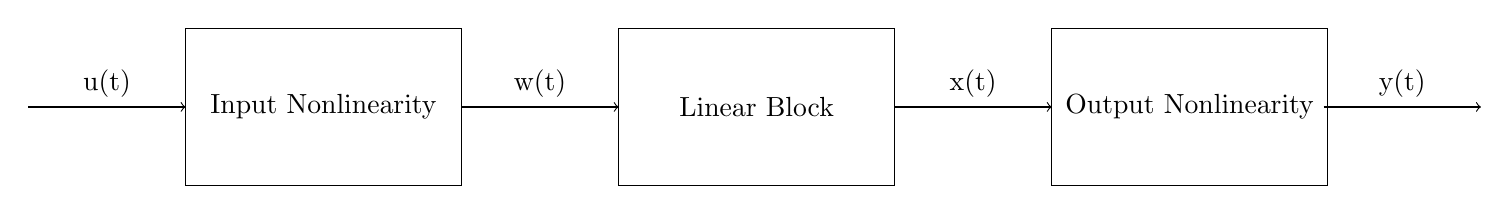
\begin{tikzpicture}
\draw  (-3.5,3) rectangle (0,1) node[pos=.5] {Linear Block};
\draw  (-9,3) rectangle (-5.5,1) node[pos=.5] {Input Nonlinearity};
\draw  (2,3) rectangle (5.5,1) node[pos=.5] {Output Nonlinearity};
\draw [->] (-5.5,2) -- (-3.5,2) node [pos=0.5,above] {w(t)};
\draw [->] (-11,2) -- (-9,2) node [pos=0.5,above] {u(t)};
\draw [->] (0,2) -- (2,2) node [pos=0.5,above] {x(t)};
\draw [->] (5.45,2) -- (7.45,2) node [pos=0.5,above] {y(t)};
\end{tikzpicture}
}
\caption{Hammerstein-Wiener model.}
\label{weiner}
\end{figure}


%\end{column}
%\end{columns}

\end{frame}



%%%%%%%%%%%%%%%%%%%%%%%%%%%%%%%%%%%%%%%%%%%%%%%%%%%%%%%%%%%%%%%%%%%%%%%%%%%%%%%%%%%

\begin{frame}{Force estimation}{Linear model}
\begin{itemize}
\item Linear model
  \begin{itemize}
  \item Choice of inputs affects model quality
  \item Inputs: effort, velocity 
  \item Outputs: force
  \end{itemize}
\item Black-box identification
	\begin{itemize}
	\item Subspace identification
	\item Hankel singular value analysis
	\end{itemize}
\end{itemize}

\end{frame}

%%%%%%%%%%

\begin{frame}{Force estimation model}{Hammerstein Wiener Models}
\begin{itemize}
  \item Nonlinearities
  \begin{itemize}
    \item Deadzone nonlinearities on input 
    \item Saturation nonlinearities on output
  \end{itemize}
\end{itemize}


 \begin{figure}[h]
 \centering
 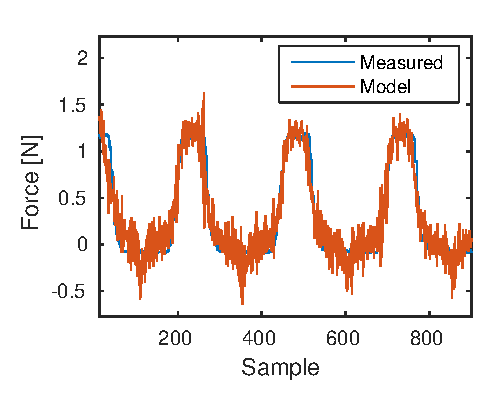
\includegraphics[width=0.49\linewidth]{modelpitch2_a}
 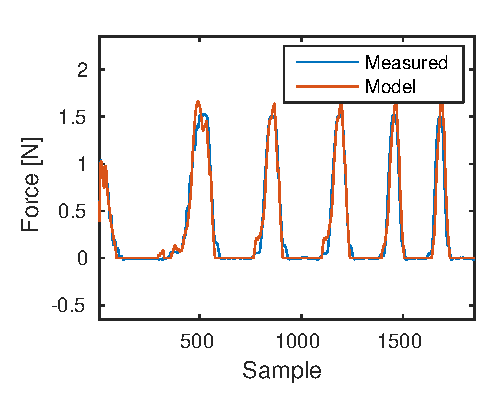
\includegraphics[width=0.49\linewidth]{modelyaw_a}
 \caption{Comparison of pitch (left) and yaw (right) model to measurements.}
 \label{fig:final_res_yaw}
 \end{figure}
\end{frame}
